\documentclass{standalone}

\usepackage{physics}
\usepackage{amsmath}
\usepackage{tikz}
\usepackage{mathdots}
\usepackage{yhmath}
\usepackage{cancel}
\usepackage{color}
\usepackage{siunitx}
\usepackage{array}
\usepackage{multirow}
\usepackage{amssymb}
\usepackage{gensymb}
\usepackage{tabularx}
\usepackage{extarrows}
\usepackage{booktabs}
\usetikzlibrary{fadings}
\usetikzlibrary{patterns}
\usetikzlibrary{shadows.blur}
\usetikzlibrary{shapes}
\newcommand{\M}{\mathbb{M}}
\usepackage{textcomp}
%\usepackage{mathpazo}
\usepackage{eulervm}
\usepackage[utf8]{inputenc}

\DeclareUnicodeCharacter{2212}{\textminus}%




\begin{document}

\tikzset{every picture/.style={line width=0.75pt}} %set default line width to 0.75pt        

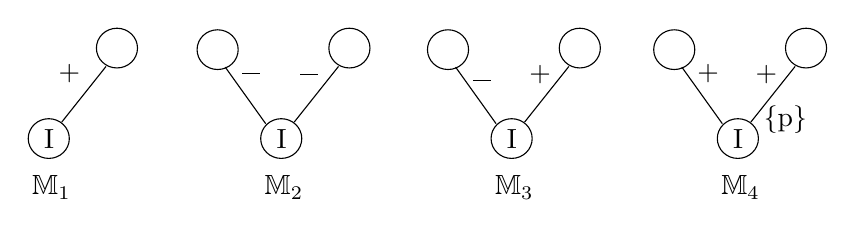
\begin{tikzpicture}[x=0.75pt,y=0.75pt,yscale=-1,xscale=1]
%uncomment if require: \path (0,300); %set diagram left start at 0, and has height of 300

%Shape: Ellipse [id:dp5119944373317229] 
\draw   (50.6,141.43) .. controls (50.6,136.15) and (55.03,131.87) .. (60.5,131.87) .. controls (65.97,131.87) and (70.4,136.15) .. (70.4,141.43) .. controls (70.4,146.72) and (65.97,151) .. (60.5,151) .. controls (55.03,151) and (50.6,146.72) .. (50.6,141.43) -- cycle ;
%Shape: Ellipse [id:dp6706693988718968] 
\draw   (83.45,97.85) .. controls (83.45,92.57) and (87.88,88.28) .. (93.35,88.28) .. controls (98.82,88.28) and (103.25,92.57) .. (103.25,97.85) .. controls (103.25,103.13) and (98.82,107.42) .. (93.35,107.42) .. controls (87.88,107.42) and (83.45,103.13) .. (83.45,97.85) -- cycle ;
%Straight Lines [id:da5562919871723839] 
\draw    (88.1,106.67) -- (66.75,133.5) ;
%Shape: Ellipse [id:dp6878885659549934] 
\draw   (162.6,141.43) .. controls (162.6,136.15) and (167.03,131.87) .. (172.5,131.87) .. controls (177.97,131.87) and (182.4,136.15) .. (182.4,141.43) .. controls (182.4,146.72) and (177.97,151) .. (172.5,151) .. controls (167.03,151) and (162.6,146.72) .. (162.6,141.43) -- cycle ;
%Shape: Ellipse [id:dp7441403778178322] 
\draw   (195.45,97.85) .. controls (195.45,92.57) and (199.88,88.28) .. (205.35,88.28) .. controls (210.82,88.28) and (215.25,92.57) .. (215.25,97.85) .. controls (215.25,103.13) and (210.82,107.42) .. (205.35,107.42) .. controls (199.88,107.42) and (195.45,103.13) .. (195.45,97.85) -- cycle ;
%Straight Lines [id:da09290279153891823] 
\draw    (200.1,106.67) -- (178.75,133.5) ;
%Shape: Ellipse [id:dp31828955727938446] 
\draw   (131.95,98.6) .. controls (131.95,93.32) and (136.38,89.03) .. (141.85,89.03) .. controls (147.32,89.03) and (151.75,93.32) .. (151.75,98.6) .. controls (151.75,103.88) and (147.32,108.17) .. (141.85,108.17) .. controls (136.38,108.17) and (131.95,103.88) .. (131.95,98.6) -- cycle ;
%Straight Lines [id:da19460803252772196] 
\draw    (145.5,107) -- (165,134.25) ;
%Shape: Ellipse [id:dp1073077218939138] 
\draw   (273.6,141.43) .. controls (273.6,136.15) and (278.03,131.87) .. (283.5,131.87) .. controls (288.97,131.87) and (293.4,136.15) .. (293.4,141.43) .. controls (293.4,146.72) and (288.97,151) .. (283.5,151) .. controls (278.03,151) and (273.6,146.72) .. (273.6,141.43) -- cycle ;
%Shape: Ellipse [id:dp01826675345857942] 
\draw   (306.45,97.85) .. controls (306.45,92.57) and (310.88,88.28) .. (316.35,88.28) .. controls (321.82,88.28) and (326.25,92.57) .. (326.25,97.85) .. controls (326.25,103.13) and (321.82,107.42) .. (316.35,107.42) .. controls (310.88,107.42) and (306.45,103.13) .. (306.45,97.85) -- cycle ;
%Straight Lines [id:da8542465891119799] 
\draw    (311.1,106.67) -- (289.75,133.5) ;
%Shape: Ellipse [id:dp6707811903815544] 
\draw   (242.95,98.6) .. controls (242.95,93.32) and (247.38,89.03) .. (252.85,89.03) .. controls (258.32,89.03) and (262.75,93.32) .. (262.75,98.6) .. controls (262.75,103.88) and (258.32,108.17) .. (252.85,108.17) .. controls (247.38,108.17) and (242.95,103.88) .. (242.95,98.6) -- cycle ;
%Straight Lines [id:da981674258758281] 
\draw    (256.5,107) -- (276,134.25) ;
%Shape: Ellipse [id:dp7484110533646813] 
\draw   (382.6,141.43) .. controls (382.6,136.15) and (387.03,131.87) .. (392.5,131.87) .. controls (397.97,131.87) and (402.4,136.15) .. (402.4,141.43) .. controls (402.4,146.72) and (397.97,151) .. (392.5,151) .. controls (387.03,151) and (382.6,146.72) .. (382.6,141.43) -- cycle ;
%Shape: Ellipse [id:dp9965994160105529] 
\draw   (415.45,97.85) .. controls (415.45,92.57) and (419.88,88.28) .. (425.35,88.28) .. controls (430.82,88.28) and (435.25,92.57) .. (435.25,97.85) .. controls (435.25,103.13) and (430.82,107.42) .. (425.35,107.42) .. controls (419.88,107.42) and (415.45,103.13) .. (415.45,97.85) -- cycle ;
%Straight Lines [id:da866391732119205] 
\draw    (420.1,106.67) -- (398.75,133.5) ;
%Shape: Ellipse [id:dp37744215237563106] 
\draw   (351.95,98.6) .. controls (351.95,93.32) and (356.38,89.03) .. (361.85,89.03) .. controls (367.32,89.03) and (371.75,93.32) .. (371.75,98.6) .. controls (371.75,103.88) and (367.32,108.17) .. (361.85,108.17) .. controls (356.38,108.17) and (351.95,103.88) .. (351.95,98.6) -- cycle ;
%Straight Lines [id:da6822079512324222] 
\draw    (365.5,107) -- (385,134.25) ;

% Text Node
\draw (57.0,135.67) node [anchor=north west][inner sep=0.75pt]   [align=left] {I};
% Text Node
\draw (84,88.53) node [anchor=north west][inner sep=0.75pt]   [align=left] {};
% Text Node
\draw (64.02,104.23) node [anchor=north west][inner sep=0.75pt]   [align=left] {+};
% Text Node
\draw (51.25,158.15) node [anchor=north west][inner sep=0.75pt]    {$\M_{1}$};
% Text Node
\draw (169.0,135.67) node [anchor=north west][inner sep=0.75pt]   [align=left] {I};
% Text Node
\draw (196,88.53) node [anchor=north west][inner sep=0.75pt]   [align=left] {};
% Text Node
\draw (179.77,104.73) node [anchor=north west][inner sep=0.75pt]   [align=left] {\textminus};
% Text Node
\draw (163.25,158.15) node [anchor=north west][inner sep=0.75pt]    {$\M_{2}$};
% Text Node
\draw (181.25,88.28) node [anchor=north west][inner sep=0.75pt]   [align=left] {};
% Text Node
\draw (151.77,104.23) node [anchor=north west][inner sep=0.75pt]   [align=left] {\textminus};
% Text Node
\draw (280.0,135.67) node [anchor=north west][inner sep=0.75pt]   [align=left] {I};
% Text Node
\draw (307,88.53) node [anchor=north west][inner sep=0.75pt]   [align=left] {};
% Text Node
\draw (290.77,104.73) node [anchor=north west][inner sep=0.75pt]   [align=left] {+};
% Text Node
\draw (274.25,158.15) node [anchor=north west][inner sep=0.75pt]    {$\M_{3}$};
% Text Node
\draw (292.25,88.28) node [anchor=north west][inner sep=0.75pt]   [align=left] {};
% Text Node
\draw (262.77,107.73) node [anchor=north west][inner sep=0.75pt]   [align=left] {\textminus};
% Text Node
\draw (389.0,135.67) node [anchor=north west][inner sep=0.75pt]   [align=left] {I};
% Text Node
\draw (416,88.53) node [anchor=north west][inner sep=0.75pt]   [align=left] {};
% Text Node
\draw (399.77,104.73) node [anchor=north west][inner sep=0.75pt]   [align=left] {+};
% Text Node
\draw (383.25,158.15) node [anchor=north west][inner sep=0.75pt]    {$\M_{4}$};
% Text Node
\draw (401.25,88.28) node [anchor=north west][inner sep=0.75pt]   [align=left] {};
% Text Node
\draw (371.77,104.23) node [anchor=north west][inner sep=0.75pt]   [align=left] {$ $+};
% Text Node
\draw (403.75,124.25) node [anchor=north west][inner sep=0.75pt]   [align=left] {\{p\}};


\end{tikzpicture}

\end{document}
